\documentclass[a4paper]{report}

\usepackage[utf8]{inputenc}
\usepackage[T1]{fontenc}
\usepackage{textcomp}
\usepackage{amsmath, amssymb}
\usepackage{xcolor}
\usepackage{tcolorbox}
\tcbuselibrary{theorems}
% Definitions & Theorems

\newtcbtheorem
  []% init options
  {definition}% name
  {Definition}% title
  {%
    colback=green!5,
    colframe=green!35!black,
    fonttitle=\bfseries,
  }% options
  {def}% prefix

\newtcbtheorem
  []% init options
  {theorem}% name
  {Theorem}% title
  {%
    colback=red!5,
    colframe=red!35!black,
    fonttitle=\bfseries,
  }% options
  {thrm}% prefix

\newtcbtheorem
  []% init options
  {example}% name
  {Example}% title
  {%
    colback=blue!5,
    colframe=blue!35!black,
    fonttitle=\bfseries,
  }% options
  {expl}% prefix

% figure support
\usepackage{graphicx}
\graphicspath{ {./images/} }
\usepackage{import}
\usepackage{xifthen}
\pdfminorversion=7
\usepackage{pdfpages}
\usepackage{transparent}
\newcommand{\incfig}[1]{%
    \def\svgwidth{\columnwidth}
    \import{./figures/}{#1.pdf_tex}
}
\DeclareMathSymbol{\lsim}{\mathord}{symbols}{"18}
\usepackage{hyperref}
\hypersetup{
    colorlinks,
    citecolor=black,
    filecolor=black,
    linkcolor=black,
    urlcolor=black
}

\begin{document}

\chapter{Set Theory}

All mathematical objects can be defined in terms of sets, and the language of set theory is used
in every mathematical subject.

\section{Definitions and the Element Method of Proof}

Sets, as defined earlier, are collections of objects, called elements. Using our new knowledge, we can
redefine some definitions.

\subsection{Subsets}

We can redefine some definitions of subsets: \[
A \subseteq B \Leftrightarrow \forall x, x \in A \to x \in B
.\] 
\[
A \not\subseteq B \Leftrightarrow \exists x  \mid x \in A \land x \not\in B
.\] 
Recall that a \textbf{proper subset} is a subset that is not equal to its containing set.

We can prove for two sets $X$ and $Y$ that $X \subseteq Y$ by \textbf{supposing} that $x$ is a particular but
arbitrarily chosen element of $X$, and \textbf{showing} that $x$ is also an element of $Y$.

\begin{definition}{Set Equality}{label}
    Set $A$ equals set $B$ if, and only if, $A \subseteq B$ and $B \subseteq A$.
\end{definition}

\subsection{Operations on Sets}

\begin{definition}{Operations}{label}
    Let $A$ and $B$ be subsets of a universal set $U$.
    \begin{enumerate}
        \item The \textbf{union} of $A$ and $B$, denoted $A \cup B$, is the set of all elements
            that are in at least one of $A$ or $B$.
        \item The \textbf{intersection} of $A$ and $B$, denoted $A \cap B$, is the set
            of all elements that are common to both $A$ and $B$.
        \item The \textbf{difference} of $B$ minus $A$ (or \textbf{relative complement}
            of $A$ in $B$), denoted $B - A$, is the set of all elements that are in
            $B$ and not $A$.
        \item The \textbf{complement} of $A$, denoted $A^c$, is the set of all elements
            in $U$ that are not in $A$.
    \end{enumerate}
\end{definition}

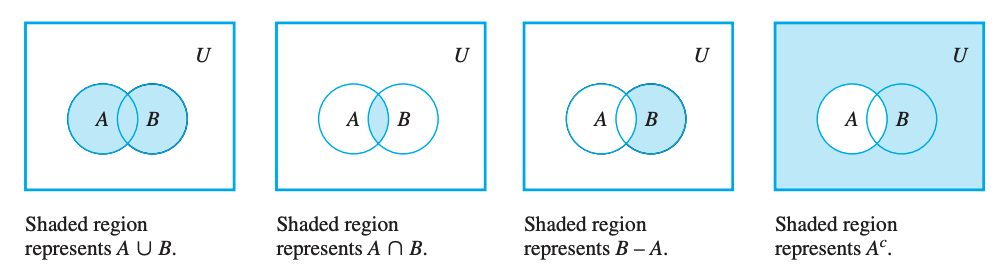
\includegraphics[scale=0.65]{setops}

\subsection{Disjoint Sets and Partitions}

A group of sets are \textbf{mutually disjoint} if the intersection of all pairs of sets is equal to
the empty set $\emptyset$.

\begin{definition}{Partition}{label}
    A finite or infinite collection of nonempty sets $\{A_1, A_2, A_3 \ldots\}$ is a \textbf{partition}
    of a set $A$ if, and only if,
    \begin{enumerate}
        \item $A$ is the union of all the $A_i$
        \item The sets $A_1,A_2,A_3 \ldots$ are mutually disjoint.
    \end{enumerate}
\end{definition}

\begin{definition}{Power Sets}{label}
    Given a set $A$, the \textbf{power set} of $A$, denoted $\wp(A)$, is the set of all subsets of $A$.
\end{definition}

\begin{definition}{Cartesian Product}{label}
    In general, \[
        A_1 \times A_2 \times \ldots A_n = \{(a_1, a_2, \ldots , a_n)  \mid a_1 \in A_1, a_2 \in A_2, \ldots , a_n \in A_n \}
    .\] 
    Note that $A_1 \times A_2 \times A_3$ is not quite the same thing as $(A_1 \times  A_2) \times A_3$
    because of tuple ordering.
\end{definition}

\section{Properties of Sets}

\begin{theorem}{Some Subset Relations}{label}
    \begin{enumerate}
        \item Inclusion of Intersection: $A \cap B \subseteq A$ and vice versa
        \item Inclusion in Union: $A \subseteq A \cup B$ and vice versa
        \item Transitive Property of Subsets: $A \subseteq B \land B \subseteq C \to A \subseteq C$
    \end{enumerate}
    To prove these theorems, \emph{suppose} that there is some arbitrary element of $A$ and show
    that it is also in $B$.
\end{theorem}

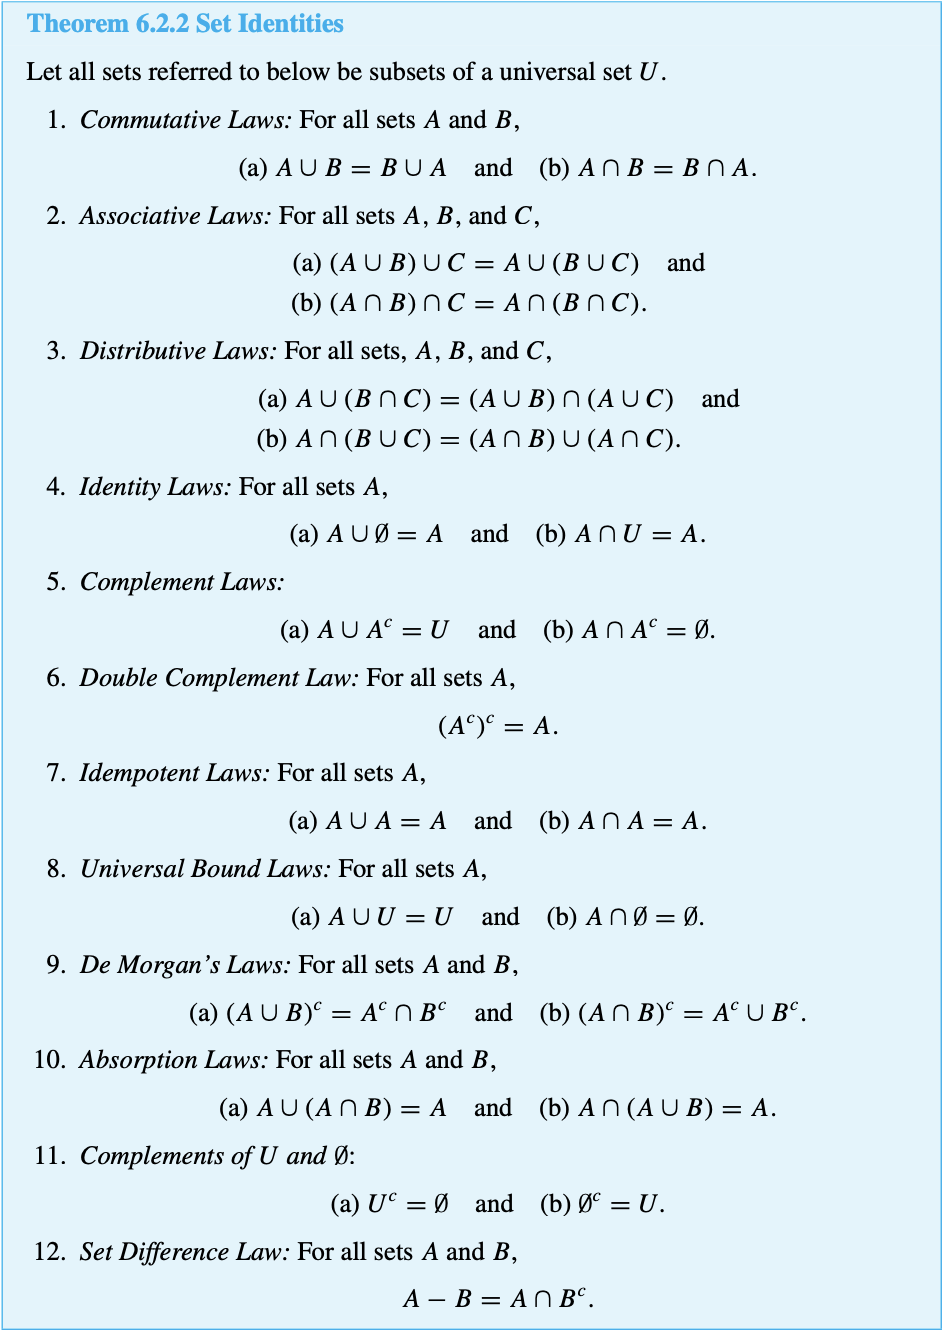
\includegraphics[scale=0.65]{setids}

In general, to prove set equality, you prove that set $A$ is a subset of set $B$, and that
set $B$ is a subset of set $A$. Additionally, to prove that a set $X$ is equal to the empty set
$\emptyset$, suppose $X$ has an element and derive a contradiction.

Additionally, casework is helpful when dealing with unions. It may be helpful to split a union into
2 cases.

\end{document}
